\documentclass{article}
\usepackage[a4paper]{geometry}
\usepackage{graphicx}
\usepackage{amsmath}
\usepackage{hyperref}

\author{Martijn Dwars (4156730) \and Rik Nijessen (4152263)}

\title{Assignment 2 \\ Software Reengineering (IN4189)}

\begin{document}

\maketitle

\section{Refactoring}
In this section we will go over the changes we made. For each change we will address the issue, explain why it is a shortcoming, how we we fixed it, and finally argue that it is indeed an improvement.

\subsection{SRP: Bug knows too much}
What is the violation and which classes/packages are involved in the violation? Why is it a shortcoming?
 -> This is a violation of SRP, because the \verb|Bug| class represents a bug but also contains functionality for retrieving bugs from the database. This is a shortcoming, because classes with many responsibilities are harder to maintain~\cite{martin2003agile}.

The refactorings you apply to resolve the violation.
 -> We implemented the Repository Pattern~\cite{repository} by creating the class \verb|BugRepository|. This class sits between the domain (i.e. \verb|Bug|) and data mapping layer (i.e. Hibernate).

Facts and arguments showing that your refactorings actually will improve the implementation and design of Alitheia Core (use diagrams, source code metrics, ...)
 -> The \verb|Bug| now solely represents a bug and the \verb|BugRepository| is responsible for loading bugs from the data layer. We were unable to find any metrics that were improved. This is probably because this change has relatively low impact.

Second SRP violation: \verb|Job| class. We split this into \verb|Job| and \verb|JobExecutor|.

\subsection{...}
...

\bibliographystyle{plain}
\bibliography{report}

\newpage
\appendix
\section{Inheritance tree} \label{app:inheritance}

\begin{sideways}
	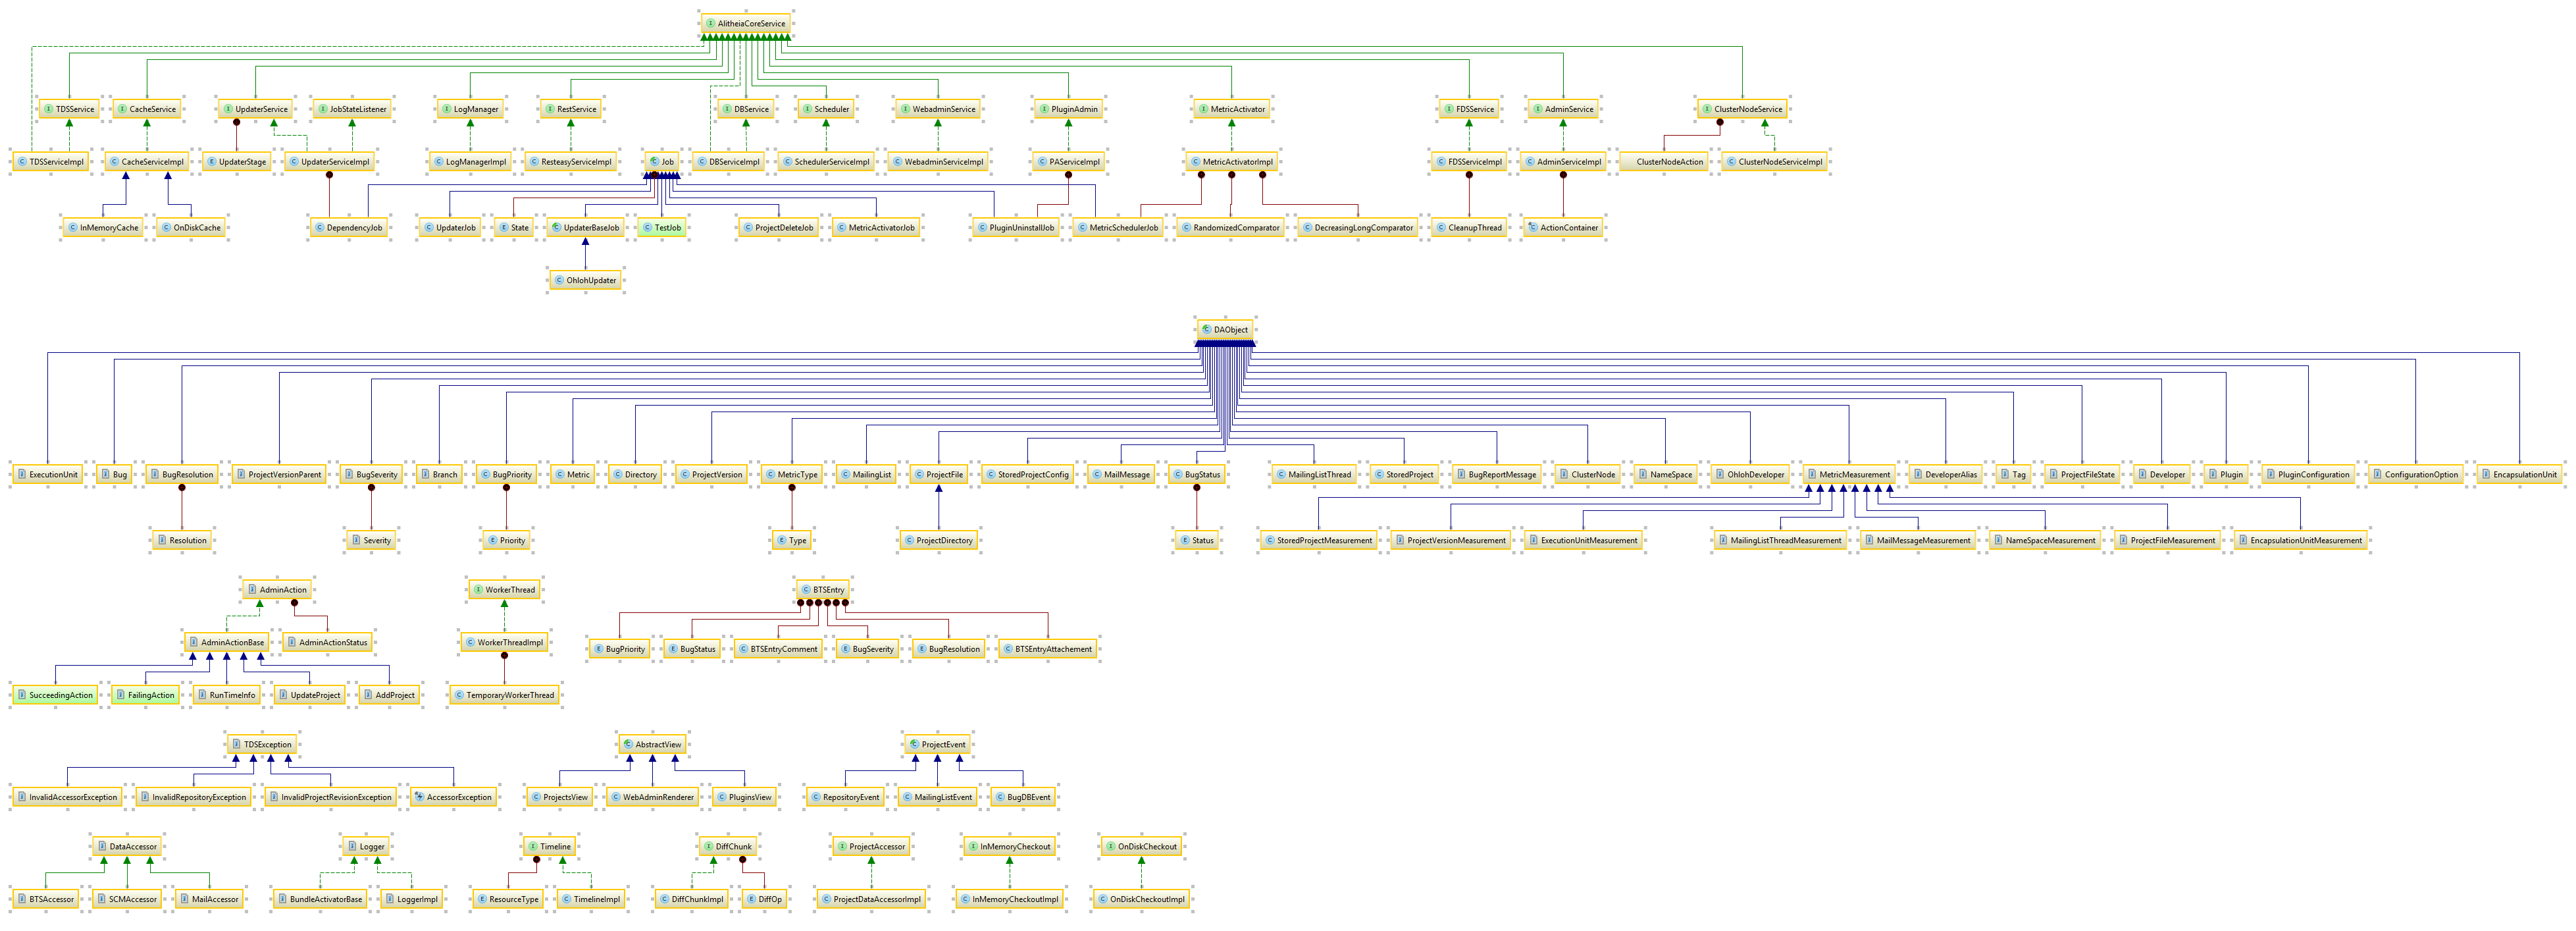
\includegraphics[width=1.3\textwidth]{inheritance-diagram}
	\label{fig:inheritance}
\end{sideways}

\end{document}